\documentclass[10pt,a4paper]{article}
\usepackage[utf8]{inputenc}
\usepackage{amsfonts}
\usepackage{graphicx}
\usepackage{indentfirst}
\usepackage{float}


\begin{document}


\title{Language Identification \\ with Contextual Translation}
\author{Alex Shah}
\date{12/4/17}


\maketitle


\section{Abstract}


This project's goal is to combine different state of the art neural network architectures to make a translator that detects the input language and translates with contextual awareness. The neural networks required to accomplish this task are a CNN classifier and tensor2tensor's transformer model for translation. Initially, this project sought to use English and Spanish languages, however due to dataset difficulties, training was done with a French dataset. It remains the case that any language with an appropriately processed dataset can be trained with these models.


\section{Introduction}


Pretrained models provide inference which reduces computation on less powerful devices since performing those costly backpropagation calculations has been done in advance. However, training the network does require a large amount of compute power and time.


In order to minimize the amount of time required, we can make training more efficient by training both translation directions simultaneously. By using encoder/decoder as a basis for our model, languages and context are broken down into mathematical representations that the network uses to translate any language to any other. We do not need to train translation from language A to language B and vice versa, but can learn each language independently. By utilizing language agnostic training, we can improve the speed at which we train. 


We store this knowledge and apply it to our problem as can be seen in Figure 2. Tensor2Tensor, the framework for machine translation in this project, works similar to Seq2Seq by mapping the words in different languages to a universal machine language allowing the model to encode and decode from the source language (regardless of the source language) to the target language.


\section{Background}


\subsection{Language Classification}


Classifying a given input is handled by a Convolutional Neural Network (CNN). It is crucial to quickly determine the input language. Identifying the language is an intermediary step before translation and incorrectly determining the input language will create incorrect translations. Therefore it is important that the classification network is able to quickly but accurately detect the input language. A CNN is accurate with very few epochs of training. In as little as 1 epoch the validation accuracy is over 99\% for inputs of 70 characters (K.M. 2016).


\subsection{Contextually Aware Translation}


Strides have been made using deep learning models for Machine Translation (MT).  MT research grows ever more accurate in contextually aware translation. Sequence to Sequence networks (Seq2Seq) are built like an encoder/decoder. The encoded input text is examined to determine the decoded output in the target language. Adding an attention mechanism is used to share information from previous input steps to better decode output. This is more efficient than bidirectionally sharing input and output values and is also more accurate than methods that require less computation such as reversing input strings. Specifically, attention shares memory between the encoder steps and decoder to produce more contextually aware output. The encoder mechanisms in NMT models are used to build a thought vector from a given input. This vector captures context which is then decoded into the target language translation. Furthermore, an attention mechanism coupled with dropout determines how much context is too little or too much. This enables the translation to capture and translate advanced syntactic structures such as gender agreement and other "long range dependencies" without overfit or poor context capture (Luong, 2015).


Neural Machine Translation (NMT) advances even further with Google's tensor2tensor library. T2T is a specifically derived set of Seq2Seq and RNN based models focusing on accuracy and efficiency of training translation models (Luong, 2015). Models like Transformer have achieved some of the best accuracies in NMT.
  
  
\clearpage


\begin{figure}[H]
  \begin{center}
    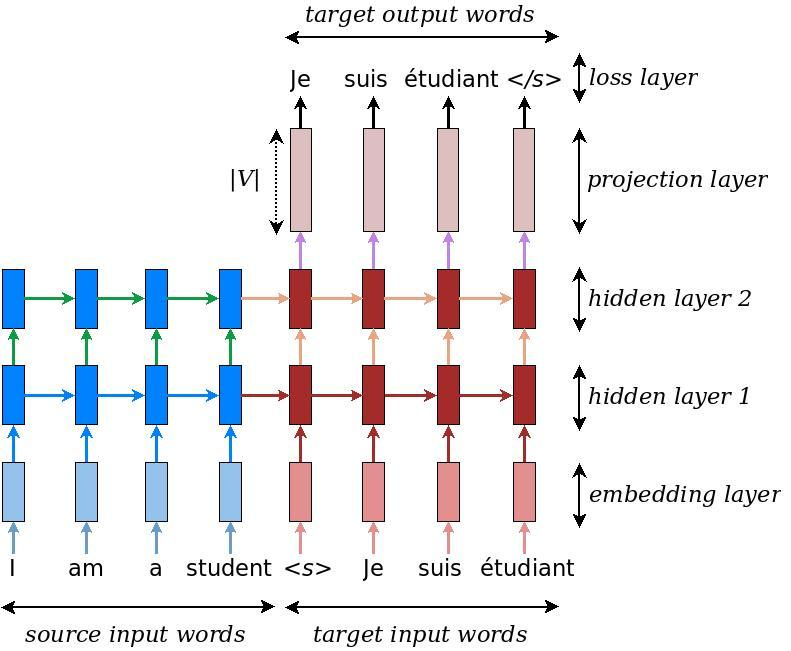
\includegraphics[width=0.9\textwidth]{seq2seq.jpg}
    \caption{Sequence to Sequence Model (Luong, 2017)}
  \end{center}
\end{figure}


\begin{figure}[H]
  \begin{center}
    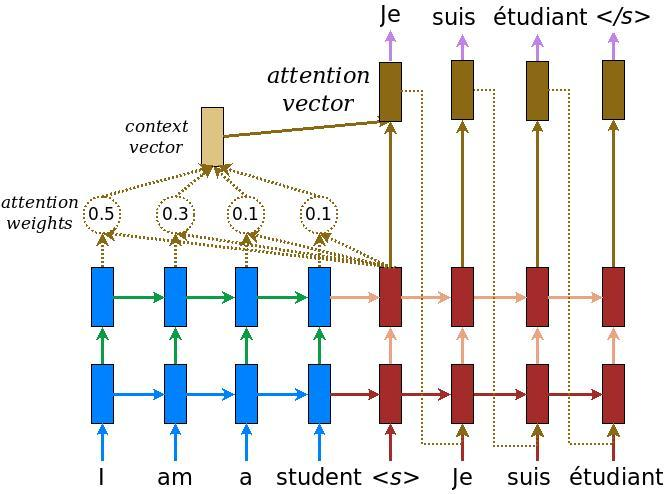
\includegraphics[width=0.9\textwidth] {attention_mechanism.jpg}
    \caption{Sequence to Sequence Model with Attention Mechanism (Luong, 2017)}
  \end{center}
\end{figure}


\clearpage


\section{Methodology}

In this project there are two networks. A Convolutional Neural Network is used as a language classifier, to detect whether a given input is English or French. Next, a tensor2tensor network, specifically using Google's Transformer model, translates the given input to the opposite language. For example a given input is identified as English and translated to French. And vice versa.
  
  
In order to improve classifier accuracy, each language’s specific characteristics are identified manually ahead of time. For example French has accented characters which allows the CNN to easily identify input characters that will only appear in a certain language (K.M. 2016).
  
  
 Transformer is the latest from Google's research into efficient and accurate multipurpose models. Transformer is able to work with a range of inputs such as images, text, and audio with a focus on scalability and efficient training. As such, transformer is able to achieve accuracy greater than previous models. In this text based project, Transformer takes in word embeddings and uses these vectorized representations of languages with multiple RNN layers wheree a feed forward encoder and an attention mechanism. The decoder also uses feed forward but while the encoder uses self-attention, the decoder is also uses source-target or encoder-decoder attention. This multihead attention is used to combat problems generalizing, namely forming relationships between different attention heads. An encoder forms a representation of the input language without needing to train translation from one language to another. The decoder translates from representations of languages to human readable output accurately and quickly (Britz, 2017).
   
   
\begin{figure}[H]
  \begin{center}
    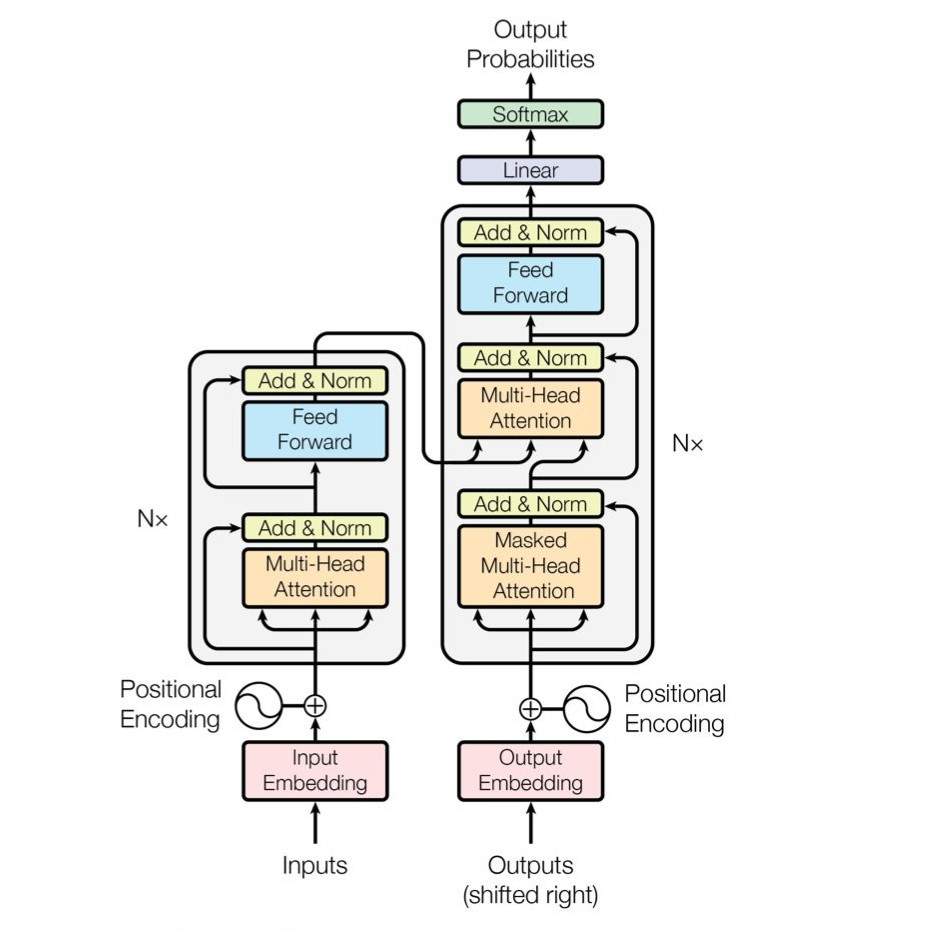
\includegraphics[width=0.7\textwidth] {transformer.jpg}
    \caption{Transformer Model architecture}
  \end{center}
\end{figure}


\clearpage


\section{Experiments}

\subsection{Classifier}
Datasets in Spanish were difficult to find, but there are many datasets in other languages. For training, the classifier and translation models were trained with the WMT17-small8k dataset in English and French. In order to train translation, the model needs to study the target language and human corrected translations. It is not necessary to train the model with the input language and human corrected translations of the target language, but rather any human corrected language. In this way a trained model can train on multiple languages without need for datasets to overlap languages, this enables us to add a new language at a later date.


The dataset is WMT's English-French small 8k vocab. This enabled both the translator and classifier to train using the same dataset. The small vocab size was necessary to train faster with a single GPU.


The classifier's CNN model was able to reach near perfect validation accuracy in the first epoch. The test accuracy after 5 epochs was 0.99, effectively not able to improve from further training.

\begin{figure}[H]
  \begin{center}
    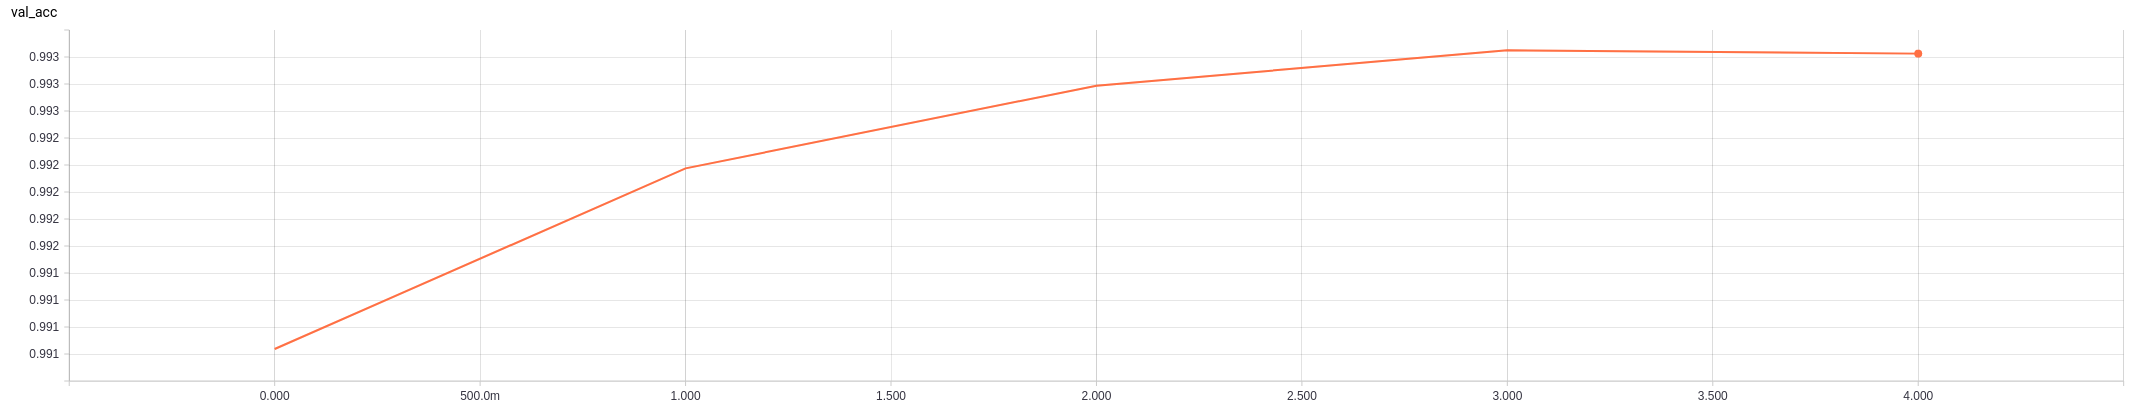
\includegraphics[width=0.9\textwidth] {val_acc1.png}
    \caption{Classifier Validation accuracy}
  \end{center}
\end{figure}

\begin{figure}[H]
  \begin{center}
    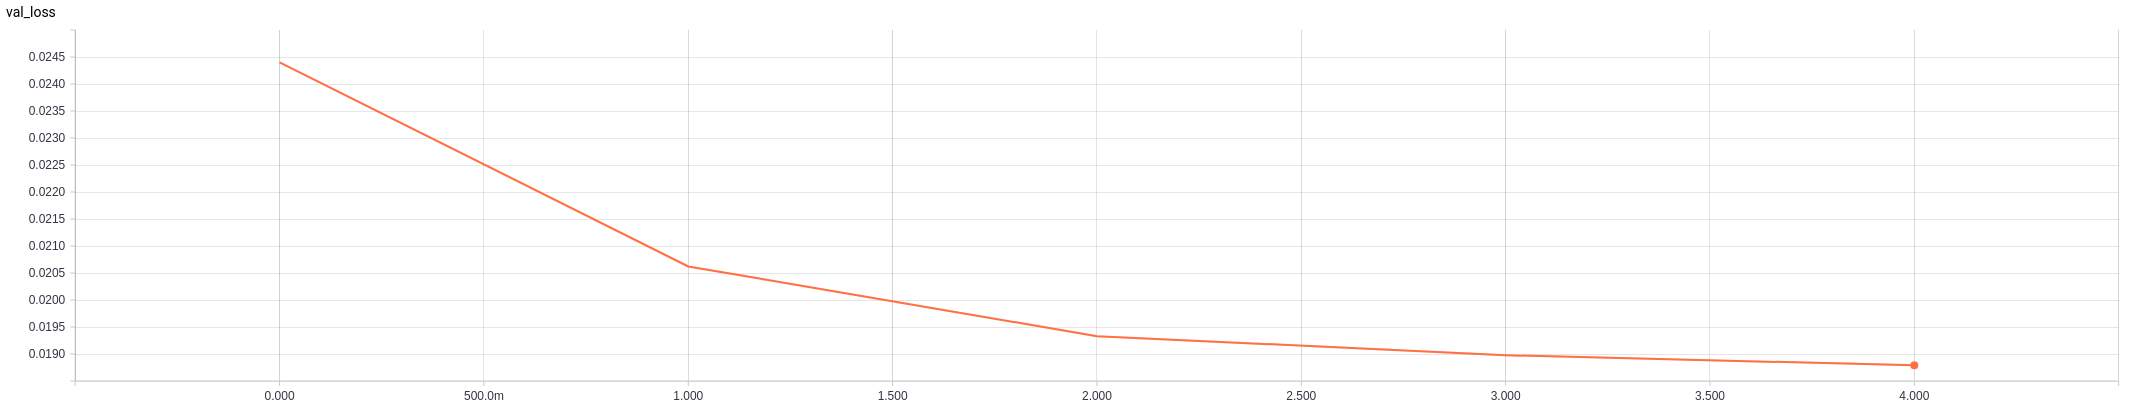
\includegraphics[width=0.9\textwidth] {val_loss1.png}
    \caption{Classifier Validation loss}
  \end{center}
\end{figure}

\clearpage

\subsection{Translation}
  
The translation net takes significantly longer to train. After 5 days, the validation estimated BLEU score was over 50. At the time of writing the estimated validation BLEU score is 51.232. Although the approximate scores showed great promise, training on a single GPU did not complete in time to run actual tests and t2t decoding could not function without reaching the target iterations. Unfortunately, training cannot be foreshortened or resumed. Therefore, while each component of the project proved to be highly accurate during training and validation steps, there was not enough time to train the translation network in time for a functional demonstration or a test version of the final product to be produced. On a single GPU (Nvidia GTX 980 Ti), the estimated time to complete training exceeds one month.


\begin{figure}[H]
  \begin{center}
    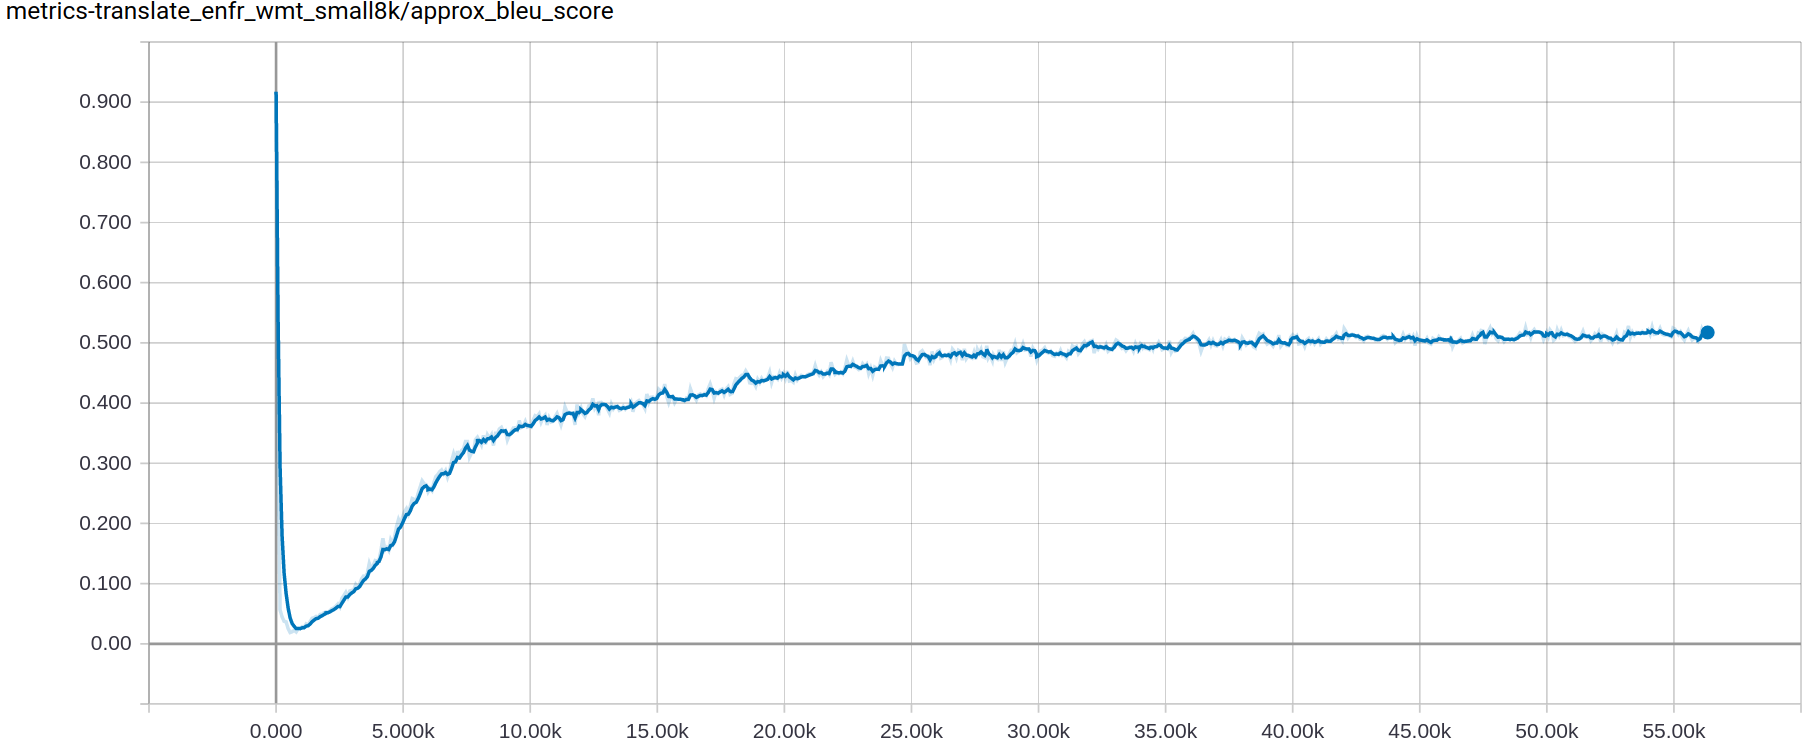
\includegraphics[width=0.9\textwidth] {BLEU.png}
    \caption{BLEU score after 5 days}
  \end{center}
\end{figure}


\begin{figure}[H]
  \begin{center}
    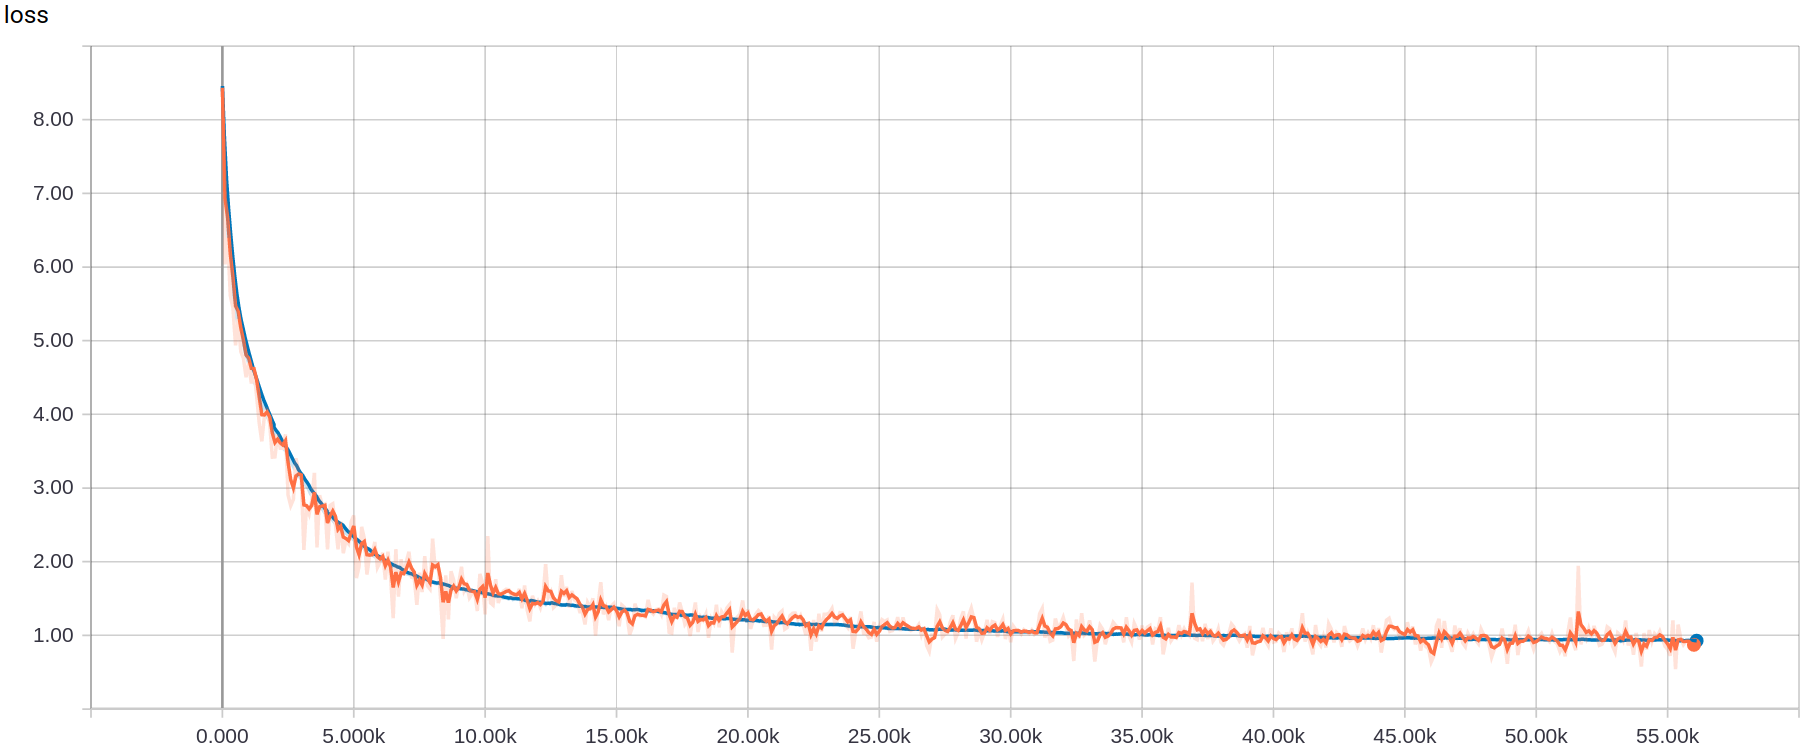
\includegraphics[width=0.9\textwidth] {loss.png}
    \caption{Loss after 5 days}
  \end{center}
\end{figure}


\begin{figure}[H]
  \begin{center}
    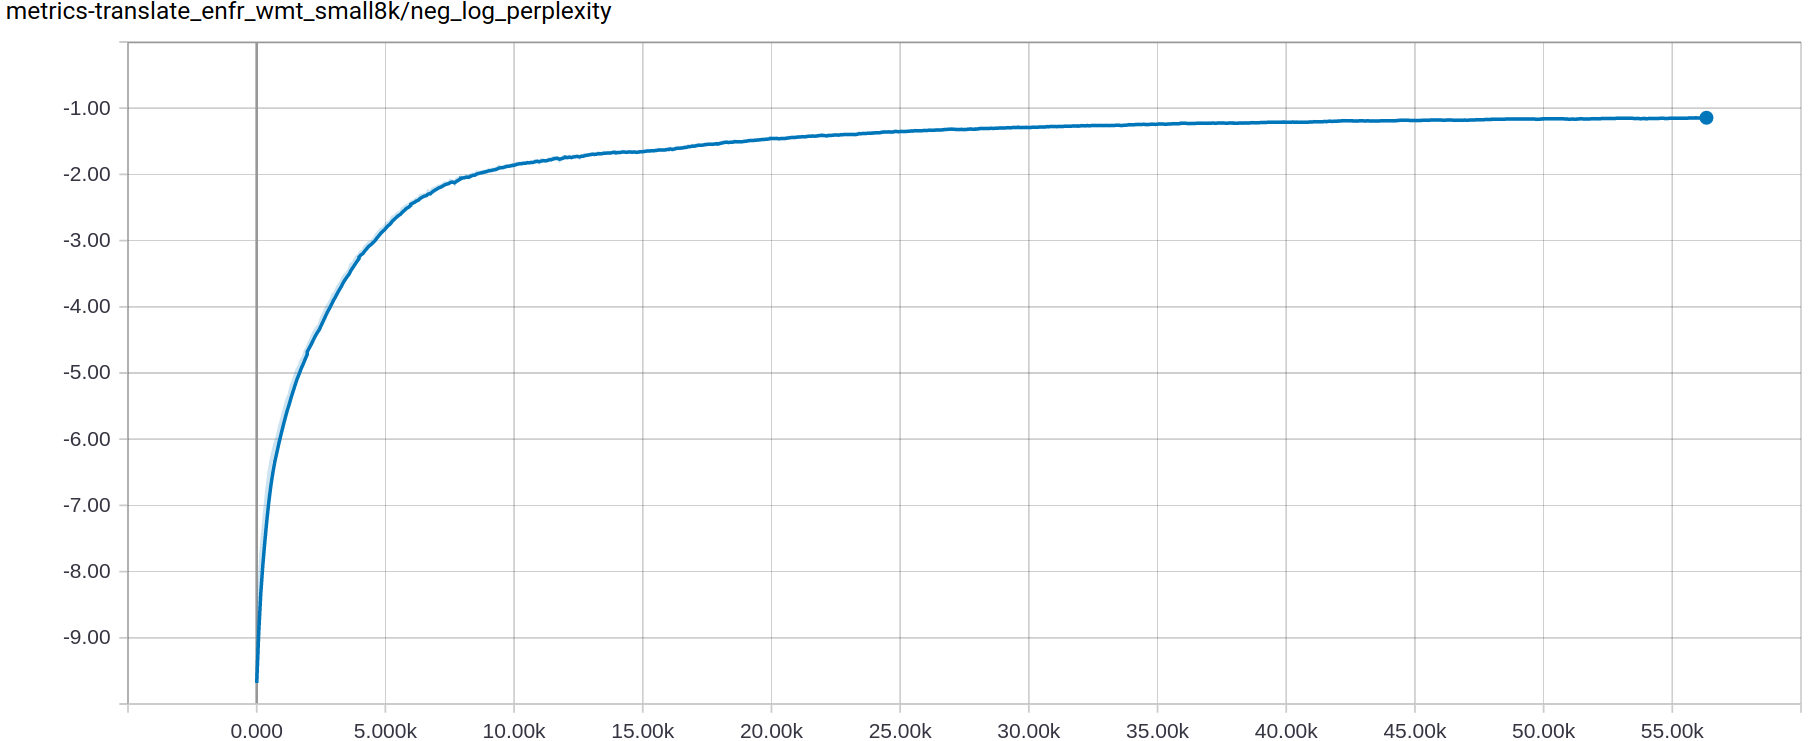
\includegraphics[width=0.9\textwidth] {neg_log_perp.png}
    \caption{Negative Log Perplexity after 5 days}
  \end{center}
\end{figure}


\section{Conclusion}


While the intention of this project was to create a finished executable, the research and training data gathered proves that the concept will work, even though training and testing was incomplete. From this project I have learned how to scale and efficiently modify basic neural network architectures, including some not so basic models, to work with particular data and concepts. The classifier works as intended to identify multiple languages. Tthe translation model will work once trained sufficiently. Training Transformer for 250,000 global steps proved to be a mistake, and what progress that was acheived could not be resumed.


\clearpage
\section{References}


\subsection{Further Reading}

https://github.com/tensorflow/nmt

https://github.com/google/seq2seq

https://github.com/tensorflow/tensor2tensor

http://www.nltk.org/

https://nlp.stanford.edu/projects/nmt/

https://research.googleblog.com/2017/07/building-your-own-neural-machine.html

https://sites.google.com/site/acl16nmt/

https://github.com/lmthang/thesis

https://google.github.io/seq2seq/data/

http://www.statmt.org/europarl/

https://conferences.unite.un.org/UNCorpus

http://www.statmt.org/wmt17/translation-task.html


\subsection{Sources}


Britz, Denny, et al. "Massive Exploration of Neural Machine Translation Architectures" Arvix, 2017.
(https://arxiv.org/pdf/1703.03906.pdf)
\newline

Johnson, Melvin, et al. "Google’s Multilingual Neural Machine Translation System: Enabling Zero-Shot Translation." Arxiv. 2016.
(https://arxiv.org/pdf/1611.04558v1.pdf)
\newline

Sutskever, Ilya, et al. "Sequence to Sequence Learning with Neural Networks." NIPS. 2015.
(https://papers.nips.cc/paper/5346-sequence-to-sequence-learning-with-neural-networks.pdf)
\newline

Cho, Kyunghyun, et al. "Learning Phrase Representations using RNN Encoder–Decoder for Statistical Machine Translation." ACLweb. 2014.

(http://aclweb.org/anthology/D/D14/D14-1179.pdf)
\newline

Bahdanau, Dzmitry, et al. "Neural Machine Translation By Jointly Learning To Align and Translate." Arxiv. 2016.
(https://arxiv.org/pdf/1409.0473.pdf)
\newline

Luong, Minh-Thang, et al. "Effective Approaches to Attention-based Neural Machine Translation." Arxiv. 2015.
(https://arxiv.org/pdf/1508.04025.pdf)
\newline

Wu, Yonghui, et al. "Google’s Neural Machine Translation System: Bridging the Gap between Human and Machine Translation." Arvix. 2016.
(https://arxiv.org/abs/1609.08144)
\newline

Neubig, Graham, et al. "Neural Machine Translation and Sequence-to-sequence Models: A Tutorial." Arvix. 2017.
(https://arxiv.org/abs/1703.01619)
\newline


\end{document}
